\chapter{Introduction}
\label{sec:intro}
\textbf{TODO}
\begin{itemize}
	\item{Explain Context in which SHAMPU was designed}
	\item{Explain Problem SHAMPU tries to fix}
	\item{Explain "Problem" of this thesis "ANT as an addition to SHAMPU, need to know how good ANT is"}
	\item{Explain how problem was solved, e.g. Different experiments which try to evaluate ANT in the context of SHAMPU}
\end{itemize}
In this thesis we evaluate the WSN testbed: SHAMPU (Single chip Host for Autonomous Mote Programming over USB). 


\section{Related work}
\label{sec:related_work}

There are already several different WSN testbeds available. These testbeds all fulfil certain roles, but ultimately fail to provide all the necessary features for a small, mobiles and low power WSN testbed.\\

There are some testbeds which need a fixed infrastructure, like FlockLab \cite{Lim2013} or Minverva \cite{Sommer}. The nature of a fixed infrastructure has certain problems. For once it might only be  viable to test inside the lab and not in the target environment since the needed infrastructure is often only available inside a lab or not easily transportable. 

Other technologies aim to detach the testbed from the infrastructure itself and rely on wireless communication instead. Sensei-UU \cite{Rensfelt2009} for example uses a wireless 802.11 network for communication between the nodes and the sensor host. The problem here is the power requirements for the communication, which makes it hard to run the nodes without an external power source.

BTNodes \cite{Moser} or Smart-Its \cite{Kasten2000} use Bluetooth to address the power issue. But Bluetooth introduces different problems, such as size limitations for the network and a difficult set-up and use of more complex network topologies. The newest version of Bluetooth tries to address this with the introduction of ScatterNets, but the setup and maintenance of the network still remains challenging.

\chapter{Technical Background}
\section{SHAMPU}
SHAMPU (Single chip Host for Autonomous Mote Programming over USB) \cite{Smeets:2014:DAL:2602339.2602401} is a WSN testbed, which allows the remote debugging and reprogramming of sensor nodes. The main advantages over other testbeds (see section~\ref{sec:related_work}) are the low cost, small size and low energy consumption. SHAMPU can be used as an extension to an already existing sensor node. The node only needs to provide an USB-Interface, SHAMPU is thus completely OS independent.
\begin{figure}[h]
\centering
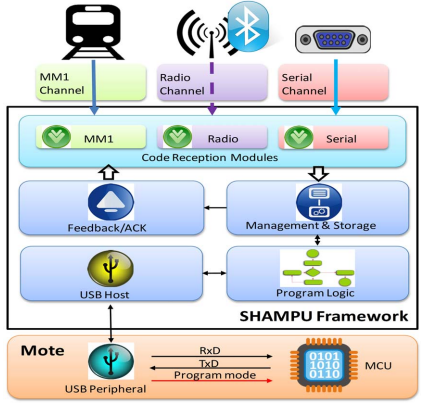
\includegraphics[scale=.5]{./pics/SHAMPUframework.png}
\caption{Overview of the SHAMPU Framework}\label{fig:shampuframework}
\end{figure}
The SHAMPU framework (see Figure \ref{fig:shampuframework}) itself is split into multiple modules. The Code Reception Module allows the use of different protocols to connect to and communicate with other SHAMPU enabled devices. For wireless communication SHAMPU uses an ANTAP1MxIB RF Transceiver Module, which supports the ANT protocol. The USB Host module is used to connect to the sensor node, which SHAMPU is attached to.

\section{ANT}
ANT \cite{DynastreamInnovationsInc.2013} is a wireless protocol which operates in the 2.4 GHz ISM Band. Originally developed in 2003 by Dynastream Innovations Inc. for the use wireless sensors. The ANT protocol is designed for the use in low power WSNs and puts a focus on scalability and ease of use.
\begin{figure}[h]
\centering
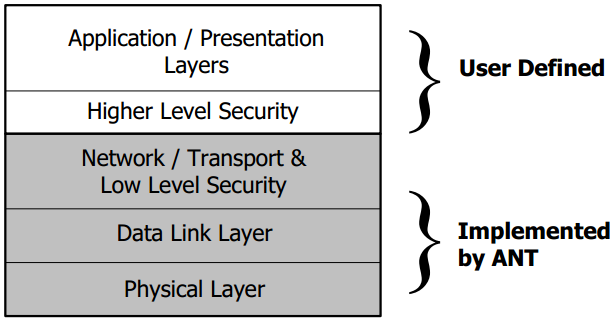
\includegraphics[scale=.5]{./pics/ANTstack.png}
\caption{OSI-Layer vs. ANT Protocol}\label{fig:osilayer}
\end{figure}
One of the advantages ANT has over other protocols, like Bluetooth or ZigBee is the high level of abstraction the ANT Protocol provides. This is achieved by the incorporation the first 4 OSI-layer (see Figure \ref{fig:osilayer}) into the ANT protocol and thus allowing even low-cost MCU to setup and maintain complex wireless networks.

\subsection{ANT Topology}

In order for ANT-Nodes to communicate with each other, they have to be part of a network. This is done be creating a channel and connection two or more different ANT nodes together. 
\begin{figure}[h]
	\centering
	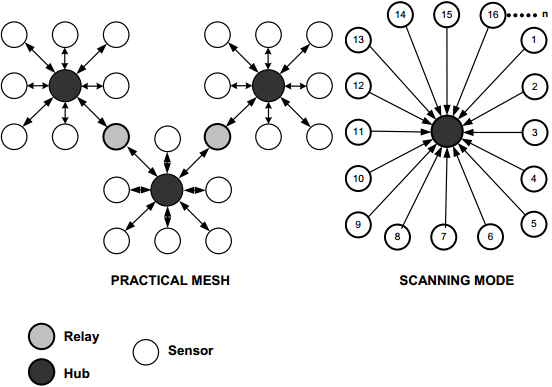
\includegraphics[scale=0.7]{./pics/ANTtopo.png}
	\caption{Example ANT Topologies}\label{fig:anttopo}
\end{figure}\\
\textbf{TODO}
\begin{itemize}
	\item{Explains what ANT nodes are}
	\item{Explain what channels are (for now in section ANT Channels)}
\end{itemize}

\subsection{ANT Channels}
Most of the available channel types are bidirectional, but the ANT protocol still differentiates between master and slaves nodes. While a master nodes mostly sends data and a slave nodes mostly receives data, the slave still has the ability to response to the incoming data.

The ANT protocol knows 125 different channels, each 1 MHz wide. Each Channel supports a data rate of 1 Mbps and up to 65533 nodes. To avoid interference between the channels isochronous selfadjusting TDMA technology is used, this allows the ANT nodes to change the transmit timings and even the frequency that is being used for the current channel.

\textit{Picture Process to establish a channel between master and slave nodes.}

The ANT protocol distinguishes between 2 different Channel types:
\begin{description}
\item{\textbf{Independent Channels}} \hfill \\ Independent Channels are used if there is only one ANT node, which is transmitting data. This allows 1:1 transmission, but also broadcasts.
\item{\textbf{Shared Channels}} \hfill \\ Shared Channels are used if a single ANT node needs to receive data from many nodes. This type of channel is made possible by the use of Shared Channel Address, however this reduces the amount of data that can be transmitted at a time.
\end{description}

\subsection{ANT Communication}
\textbf{TODO}
\begin{itemize}
	\item{Explain how each msg is structured}
	\item{Explain extended msg }
\end{itemize}

\section{ANTAP1MxIB RF}
In order to use the ANT protocol each SHAMPU-mote is equipped with an ANTAP1MxIB RF Transceiver Module. The module was chosen because of it's small form factor (20mm x 20mm) and very low power draw. The ANTAP1M can handle up to 4 ANT channels and a 1Mbps RF data rate, which is enough to setup and use the desired network topology.

\textbf{TODO}
\begin{itemize}
	\item{Explain how the Chip communicates with the SHAMPU node}
	\item{Explain how the Chip communicates with the host PC}
\end{itemize}

\chapter{Evaluation of SHAMPU}
In order to assess the capabilities of SHAMPU we plan and run experiments designed to evaluate the SHAMPU framework in the following three categories:
\begin{itemize}
	\item{\textbf{Communication Range}} 
	\item{\textbf{Communication Delay}} 
	\item{\textbf{Data Throughput}} 
\end{itemize}

For this we designed different scenarios, which test one or more of the described categories. The following section describes the experiments according to the following template:

\begin{description}
\item{\textbf{Name}} \hfill \\ The name of the experiment.
\item{\textbf{Description}} \hfill \\ A description of the experiment and the the category being evaluated.
\item{\textbf{Network Topology}} \hfill \\ A diagram of the network topology in which the experiment is run.
\item{\textbf{Result}} \hfill \\ The results of the experiment and any additional collected data.
\end{description}


\section{Experiment 1: Delay calculations between two nodes}

\section{Experiment 2: Delay calculations between multiple nodes}

\section{Experiment 3: Maximal communication Range}
\textit{Diagram for the experiment:  2 nodes   x meter apart.  with distances from 0.5 m to 30m  (floor in SM 3xx is 27m long)}
In this experiment we propose to test this theoretical limit, we set up two ANT radios next to each other. We then start moving the nodes away from each other until the connection breaks. We then start moving the nodes back together until a new connection is established.

\section{Experiment 4: Data Transfer between two nodes}
The ANT protocol promises a speed of up to 1 Mbps, 20 kbps of which are available for the application itself. In this experiment we try to determining the speed with which it is possible to move data to and form a SHAMPU device. We also try to determinate what effect the size of the payload and the number of the nodes in the network have on the transmission speed.

\section{Experiment 5: Reflash of a wireless sensor network}

\chapter{Conclusion}
\textbf{TODO}
\section{Summary}
\textbf{TODO}
\section{Future Work}
\textbf{TODO}
